\subsection{Parallélisation des méthodes itératives}
La partie résolution de système linéaire creux représente souvent la partie qui consomme le plus de temps dans une simulation numérique, par exemple dans la simulation de réservoir cela peut représenter jusqu'à 80~\% du temps de simulation.
%
Il est donc essentiel de paralléliser cette partie du code.
%
Les noyaux de calcul les plus coûteux du GMRES préconditionné sont :
\begin{itemize}
  \item la factorisation ILU;
  \item les résolutions triangulaires;
  \item le produit matrice vecteur creux;
  \item les produits scalaires.
\end{itemize}

La méthode parallélisation la plus répandue du GMRES est la méthode de Jacobi par blocs.
%
Dans cette méthode, nous découpons des blocs dans la matrice et nous appliquons notre préconditionneur sur chaque bloc.
%
Ces blocs proviennent d'un partitionnement du graphe d'adjacence~\ref{fig:domain} de la matrice à l'aide d'un logiciel de partitionnement, tel que Scotch ou Metis, avec pour objectif un bon équilibrage de charge.
%
La matrice est ensuite réordonnée pour que la numérotation des cellules à l'intérieur d'un domaine soit contiguës.
%
Ces domaines formeront des blocs dans la matrice~\ref{fig:domain_jacobi} sur lesquels nous appliquerons notre préconditionneur ILU.
%
Avec autant de blocs que de coeurs de calcul, nous pouvons factoriser tous les blocs parallèlement.
%
Cette méthode ignore donc les interactions inter-domaine et fournit donc un bon préconditionnement.


\begin{figure}[!h]
     \begin{center}
        \subfigure[Exemple d'une décomposition en quatre domaines.]{
          \label{fig:domain}
          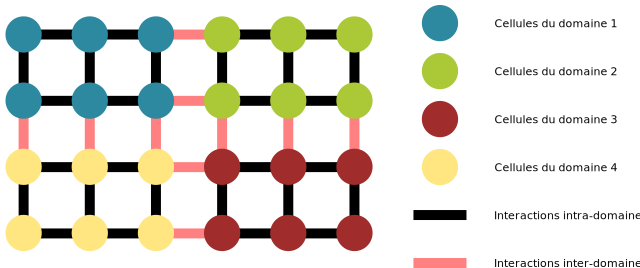
\includegraphics[width=\textwidth]{domain}
        }
        \subfigure[Une matrice ordonnée par domaine. Les entrées en dehors des carrées seront ignorées lors de la factorisation ILU.]{
          \label{fig:domain_jacobi}
          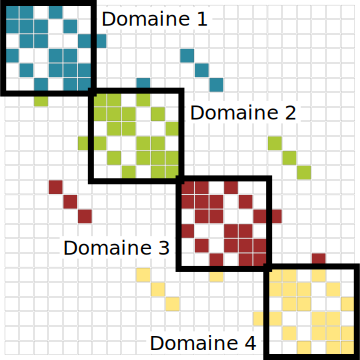
\includegraphics[width=0.50\textwidth]{domain_jacobi}
        }
    \end{center}
    \caption{.}
    \label{fig:jacobi}
\end{figure}
